\chapter{厂商的要素选择}
\label{chp:producer-choice}

\section{既定产量下的成本最小化}
\label{sec:cost-minimization}

\begin{equation}
\begin{split}
\min c &= wl + rk\\
\text{s.t.~} q^* &= f(l,k)
\end{split}
\end{equation}

如果任何一种要素价格上升则最小成本必上升:如果一种要素变得更贵而另外一种要素的价格不变,最小成本不可能下降,一般会上升\footnote{%
Varian, H. R. (2010). \emph{Intermediate Microeconomics A Modern Approach} (8 ed.). W. W. Norton: 369.};类似地,如果企业决定生产更多的产量而且所有要素价格维持不变,则企业的成本必然上升。

\begin{figure}[!h]
\colorbox{black!3}{\parbox{\linewidth-2\fboxsep}{%
\centering
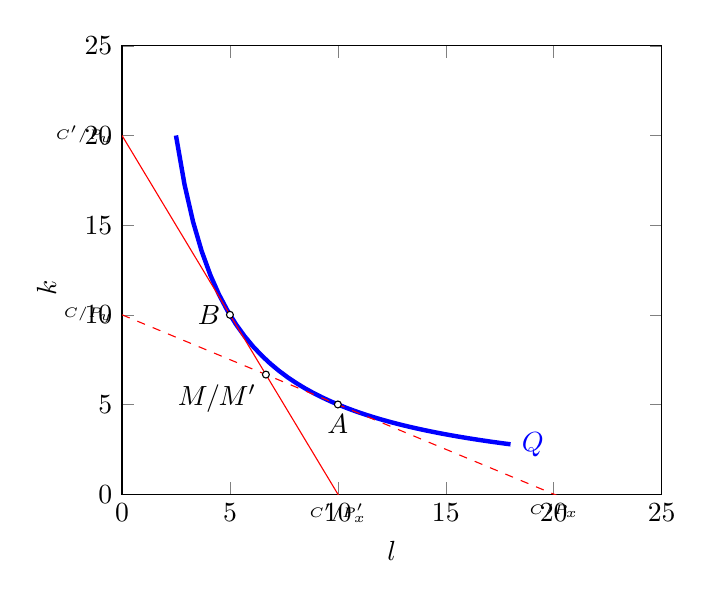
\begin{tikzpicture}
\begin{axis}[
	xmin=0,xmax=25,ymin=0,ymax=25,
	xlabel style={below},xlabel=$l$,
	ylabel style={left},ylabel=$k$,
	extra x ticks={10,20},
	extra x tick style={tickwidth=0},
	extra x tick labels={{\tiny$C'/{P'_x}$},{\tiny$C/{P_x}$}},
	extra y ticks={10,20},
	extra y tick style={tickwidth=0},
	extra y tick labels={\tiny$C/P_y$,\tiny$C'/P_y$},
	samples=40]
\addplot[blue,ultra thick,domain=2.5:18]
		{50/x} node[right] {$Q$};
\addplot[red,domain=0:25]
		{20-2*x};							%涨价之后的预算线
\addplot[red,dashed,domain=0:25]
		{10-0.5*x};
\addplot[only marks,forget plot,black,mark options={mark size=1.25pt,fill=white},mark=*] coordinates {
	(10,5)
	(20/3,20/3)
	(5,10)};
\node[below] at (axis cs:10,5) {$A$};
\node[left] at (axis cs:5,10) {$B$};
\node[below left] at (axis cs:6.667,6.667) {$M/M'$};
\end{axis}
\end{tikzpicture}
\caption{产量不变,一种要素价格上涨,总成本上涨}
}}
\end{figure}

\section{既定成本下的产量最大化}
\label{sec:production-maximization}

\begin{equation}
\begin{split}
\max q &= f(l,k)\\
\text{s.t.~} c^* &= wl + rk
\end{split}
\end{equation}

\section*{推荐阅读}
\markright{推荐阅读}
\addcontentsline{toc}{section}{\hspace{-2.5em}推荐阅读}
